\section*{8. Norms and Norm Dependent Linear Regression}
\subsection*{Norms}
\begin{itemize}
    \item
        The function $\norm{\cdot}$ is called a norm if it
        \begin{enumerate}
            \item
                is nonegative: $\forall x: \norm{x} \geq{0}$
            \item
                is definite: $\norm{x} = 0$ only if $x = 0$
            \item
                is homogeneous: $\norm{ax} = |a| \cdot \norm{x}$ where $a \in \mathbb{R}$
            \item
                fulfills the triangle inequality: $\forall x,y: \norm{x+y} \leq \norm{x} + \norm{y}$
        \end{enumerate}
    \item
        $L_p$-norm ($p>0$) of a d-dimensional vector is defined as $$\norm{x}_p = (\sum_{i=1}^{d} |x_j|^p)^{\frac{1}{p}}$$
        \begin{itemize}
            \item
                $L_0$-norm denotes number of non-zero entries
            \item
                $L_1$-norm: $\norm{x}_1 = \sum_{i=1}^d |x_i|$ (sum of absolute values)
            \item
                $L_2$-norm: $\norm{x}_2 = (\sum_{i=1}^d x_i^2)^{\frac{1}{2}}$ (sum of squared values)
            \item
                $L_{\infty}$-norm: $\norm{x}_{\infty} = \underset{i}{max}\{|x_i|; i=1,2,\dots,d\}$
        \end{itemize}
    \item
        Quadratic $L_{\textbf{P}}$-norm, where $\textbf{P}$ is a positive definite matrix: $\norm{x}_{\textbf{P}} = \norm{\textbf{P}^{\frac{1}{2}}x}_2$
    \item
        Mahalanobis distance: $\norm{x-y}_{\Sigma^{-1}} = \sqrt{(x-y)^T \Sigma^{-1} (x-y)}$
    \item
        Unit ball: $B = \{x | \norm{x} \leq 1\}$
    \end{itemize}

    \begin{figure}[H]
        \centering
        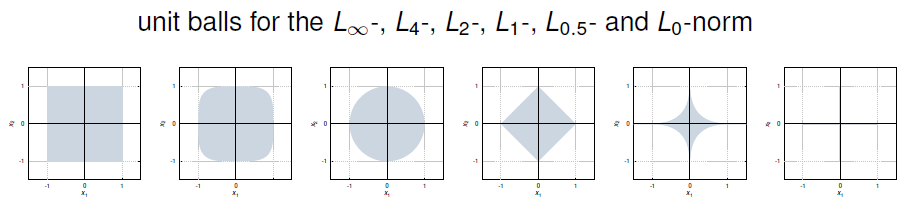
\includegraphics[scale=0.8]{figures/unit_ball}
    \end{figure}

\begin{itemize}
    \item 
        Frobenius norm: $\norm{X}_F = \sqrt{\sum_{i=1}^m \sum_{j=1}^n x_{i,j}^2}$
    \item
        A norm is a measure for the length of a vector or a measure of distance: $dist(x,y) = \norm{x-y}$
\end{itemize}

\subsection*{Norm Dependent Linear Regression}
\begin{itemize}
    \item
        General norm dependent linear regression problem: minimize $\norm{Ax - b}$ or $\hat{x} = \underset{x}{argmin} \norm{Ax - b}$
    \item
        Different norms lead to different results, range from closed form solution to LP-problem
    \item
        The estimation error $e \in \mathbb{R}$ is defined by $e = \norm{x^* - \hat{x}}$, where $x^*$ denotes the correct value
    \item
        The residual $r=(r_1, r_2, \dots, r_m)^T$ is defined by $r = Ax -b$ 
\end{itemize}
\subsection*{Ridge Regression/Lasso and Unit Balls}
\begin{figure}[H]
    \centering
    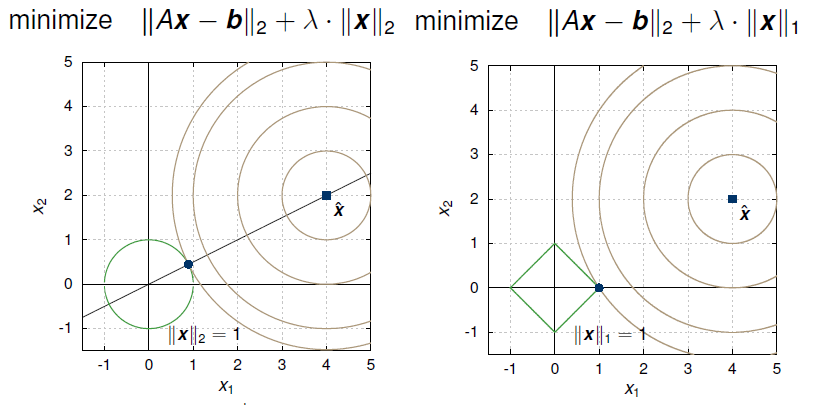
\includegraphics[scale=0.6]{figures/ridge_lasso}
    \caption{Left: Ridge Regression, Right: Lasso}
\end{figure}
\subsection*{Penalty Function}
\begin{itemize}
    \item
        The penalty function approximation problem is defined as follows:
        \begin{align*}
            \text{minimize } & \sum_{i=1}^m \phi(r_i)\\
            \text{subject to } & r=(r_1,r_2,\dots,r_m)^T = Ax-b
        \end{align*}
        where $\phi: \mathbb{R} \rightarrow \mathbb{R}$ is the penalty function for the components of the residual vector
    \item
        The penalty function $\phi$ assigns costs to residuals
    \item
        If $\phi$ is a convex function, the penalty function approximation problem is a convex optimization problem
\end{itemize}
\begin{figure}[H]
    \centering
    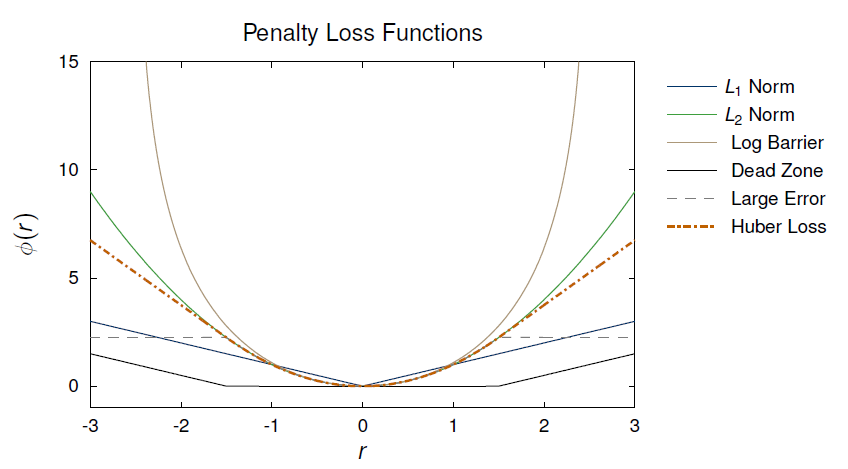
\includegraphics[scale=0.7]{figures/penalties}
\end{figure}

